\section{Tracing}

\begin{frame}
   {The Linux Tracing Infrastructure}

   \begin{itemize}
      \item
      Log not only \textbf{what} happened but also \textbf{when} it
      happened.
      \item
      Provides a rich set of \textbf{software events} (points of code)
      in the kernel.
      \item
      Custom kernel events can be added to a live system.
      \item
      Custom userspace events can be added to a live system. (Userspace
      tasks must be started after the events are added, but the programs
      do not need to be modified.)
      \item
      Tools are available to simplify usage, such as \textbf{trace-cmd}
      and \textbf{perf}.
      \item
      Graphical tools are available to view and analyze trace data, such
      as \textbf{kernelshark} and \textbf{Trace Compass}.
   \end{itemize}

\end{frame}

\cprotect\note{

   The Linux tracing infrastructure has many more features than presented
   here. With it, the possibilities for debugging and
   analyzing real-time software are nearly limitless. If you are
   serious about debugging real-time issues, it is worth it to look
   deeper into these Linux features.

   Keep in mind that this is not just for debugging. With the tracing
   infrastructure developers and testers can \textbf{verify} real-time
   performance.

   \textbf{Simple Examples:}

   List all supported events:
   \begin{raw}
trace-cmd list
   \end{raw}

   Record all the scheduling wakeup an switch events on the system
   over 5 seconds:
   \begin{raw}
trace-cmd record -e sched:sched_wakeup -e sched:sched_switch sleep 5
   \end{raw}

   View the recorded events (recorded in \texttt{trace.dat}):
   \begin{raw}
trace-cmd report
   \end{raw}

   Graphically view the recorded events:
   \begin{raw}
kernelshark
   \end{raw}

}

\begin{frame}
   {kernelshark Output}

   \begin{figure}[H]
      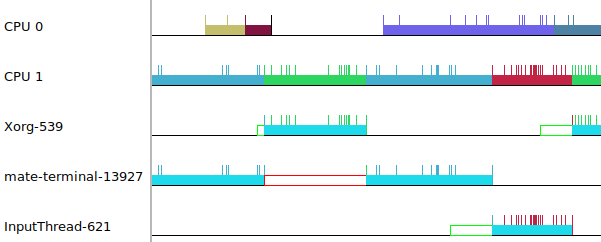
\includegraphics[width=6in]{IMAGES/kernelshark1}
      \caption{kernelshark: Scheduling overview.}
   \end{figure}

\end{frame}

\cprotect\note{

   In this figure we see that mate-terminal had work to do (is in the \texttt{RUNNABLE}
   state) but Xorg has the CPU. And CPU0 is idle!

   Is this a problem? Why do we have this situation? From the trace we do not know
   the answers to these questions. But at least we know it is happening!

}

\begin{frame}
   {kernelshark Output}

   \begin{figure}[H]
      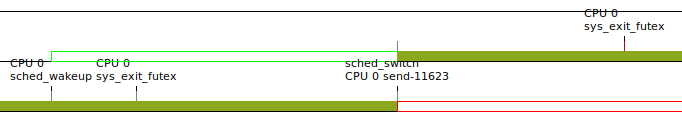
\includegraphics[width=6in]{IMAGES/kernelshark2}
      \caption{kernelshark: Scheduling details.}
   \end{figure}

\end{frame}

\cprotect\note{

   From a detailed (zoomed in) view, we can measure the latences between
   when the task is set \texttt{RUNNABLE}, when it started running on the
   CPU, and when it returned to userspace.

   In most cases there is no need for expensive hardware solutions. The
   kernel comes with all these features built-in!

}
